\documentclass[11pt,a4paper]{ivoa}
\input tthdefs
\usepackage{todonotes}
\usepackage{array}


\usepackage{graphicx}

\newcommand{\dataciteterm}[1]{\colorbox{lightgray}{DataCite:\textbf{#1}}}
\newcommand{\important}[1]{
	\begin{bigdescription}
		\item \color{ivoacolor}\textbf{Note} #1
	\end{bigdescription}
}




\title{Best practices for the creation of and metadata for digital object identifiers in astronomy archives}

% see ivoatexDoc for what group names to use here; use \ivoagroup[IG] for
% interest groups.
\ivoagroup[IG]{Data Curation and Preservation}

\author[https://orcid.org/0000-0003-0666-6367]{August Muench}
\author[]{Gilles Landais}
\author[]{Raffaele D'ABrusco}
\author[]{Anne Raugh}

\editor{TBD}

% \previousversion[????URL????]{????Concise Document Label????}
\previousversion{This is a draft}


\begin{document}
\todo{This is only an outline! Everything is still to be done.}

\begin{abstract}
Many astronomy archives are producing digital object identifiers (DOI) for datasets and services.
This document aims to summarize current workflows for creating and using DOIs, 
diagnose issues in the metadata of extant DOIs, 
and develop best practices for worklows and metadata for future DOI deployment.
This note is focused on archives in Astronomy, Planetary Science, and Heliophysics. 
Additional domains may be considered at a later time.
\end{abstract}


%-------------------------------------------------------------------------------------------
\section*{Acknowledgments}

???? Or remove the section header ????

%-------------------------------------------------------------------------------------------
\section*{Conformance-related definitions}

The words ``MUST'', ``SHALL'', ``SHOULD'', ``MAY'', ``RECOMMENDED'', and
``OPTIONAL'' (in upper or lower case) used in this document are to be
interpreted as described in IETF standard RFC2119 \citep{std:RFC2119}.

The \emph{Virtual Observatory (VO)} is a general term for a collection of federated resources that can be used to conduct astronomical research, education, and outreach.
The \href{https://www.ivoa.net}{International Virtual Observatory Alliance (IVOA)} is a global collaboration of separately funded projects to develop standards and infrastructure that enable VO applications.


%-------------------------------------------------------------------------------------------
\section{Introduction}
\label{sec:intro}
\todo{Known major missing pieces: Explicit DataCite metadata keywords; Guidance on DataCite deposit, including JSON markup or Fabrica.  }

\subsection{General observations} 
\textbf{\color{red} this section was in 1.Introduction, items 1+2}

We focus on roles of digital object identifiers (DOIs) rather than the full landscape of FAIR data \citep[e.g.,][]{Wilkinson2016}. 
It is beyond the scope of this document to address all aspects of FAIRness.
It is also unreasonable we think for DOIs to be laden with the problems of enabling all aspects of FAIRness. 
Instead we aim for this document to guide archives with achieve compliance for specific aspects of enabling FAIR data.


In this document we are using DataCite Commons  \footnote{\url{https://commons.datacite.org}}. This document adopts DataCite Metadata Schema 4.5.
We choose relevant examples from existing DOI taken in approximatively 75000 dataset DOIs in astronomy (See Table \ref{tab:astroDOIs1}). 



\subsection{DOI landscape}
\textbf{\color{red}This section has been added by Gilles}
%The DOI usage is confirmed in Open Science, it opens the door to a large audience by improving citation and traceability of data. 

It is now in the landscape that the publishing of scientific articles has included DOIs in its process. A good DOI curation allows to provide standard metadata that can be harvested and reused to generate citation with authors and any information required for a bibtex. It includes references and related products that build step by step a graph of linked resources.

%The DOI is in the article publication process which generate DOI for each publication and links references to other sources. It allows to link Data with articles and draw the basis for an interconnected architecture that allows to trace the usage and origin of Data published.
DOIs are widely used for data, and although their metadata is slightly different from articles, they work very well together.


The DOI is a sustainable identifier applied to a web resource that emerge today among other identifier such  as the ORCID\footnote{\url{https://orcid.org/}}, for authors, the RoR\footnote{\url{https://ror.org/}} for organization or the RAID\footnote{\url{https://raid.org/}} for projects.

The DOI success is a consequence of an architecture that includes URL resolution (since each DOI is attached to a landing page) and standardized metadata that provides exploitable information. As a unique and standard identifier it allows to make the bridge between different networks which complete each others (more details in \ref{sec:bestpractice:providing})
%For instance, the registry of the Virtual Observatory is dedicated to link resource with services using the IVOID\footnote{\url{https://www.ivoa.net/documents/IVOAIdentifiers/}} identifier but is role is not adapted for citation.\note{redundancy with 4.1.1}

Data Centers motivated for citation and interconnection, must curate relevant metadata. 
In this document, we will develop a good practices to provide well citation, interconnections with related resources, including IVOA resources.


\subsection{Use case}
\textbf{\color{red}This section has been added by Gilles}

\begin{enumerate}
	\item Authors and Data Center expect that the resources they created or provide will be included in the citations of each article or resources which used them. It needs well curated Bibtex, linking the Data. Users expect also a visible Bibtex in the Data Center web pages.
	
	\item The Data consumer expects to get information about origin and rights. For access rights, existing license must be visible but also readable by software.
	
	\item Data published are disseminated in networks like the VO registry, DatasetSearch or the EOSC EU node (see \ref{sec:bestpractice:providing}). The users as well as the Data Center expect that the entries are consistent.
	
	\item The Data Center as well as authors needs reports about the usage activity of their work. They query dedicated services (eg: OpenCitation) that make reports and are capable to graph the citation of a specific resource.
	
	\item a workflow using external resource would execute again a process. It expects that the experience is reproducible. If it uses a service or Knowledgebase, it expects that the protocols stay compatible with the original implementation. For Dataset, it could expects that data have not been altered. 
	
	
	%%reproducibility (not possible with evolving dataset, eneous with service,hors-contexte pour KD)
\end{enumerate}

\subsection{Example of existing DOI}
\textbf{\color{red} this section was in the original 1.Introduction}


This list is not exhaustive; see Table XXX in Appendix A for a complete listing. 

\begin{table}[th]
\begin{tabular}{lclcr}
\sptablerule
\textbf{Archive} & \textbf{Prefix} & \textbf{ID} & Yo & \textbf{Count} \\
\sptablerule
Canadian Astronomy Data Centre        & 10.11570 & nrc.cadc        & - &     80   \\
Chandra Data Archive                  & 10.25574 & si.cda          & - & 29,449   \\
ESO Science Archive Facility          &          &                 & - &          \\
European Space Agency                 & 10.5270  &                 & - & 28,858   \\
IPAC (26131 --- 26135)                & 10.2613X & caltech.ipacdoi & - &    622   \\
Mikulski Archive for Space Telescopes & 10.17909 & stsci.mast      & - &  2,132   \\
NASA Planetary Data System            & 10.17189 & nasapds.nasapds & - &  1,976   \\
++Small Bodies Node of PDS            & 10.26007 & sbn.archive     & - &  4,837   \\
Strasbourg Astronomical Data Center   & 10.26093 & inist.cds       & - & 17,383   \\
\sptablerule
\end{tabular}%
\caption{\label{tab:astroDOIs1}}
\end{table}


\begin{admonition}{Note}
Dataset DOIs do not lead to data, or what they do lead to is widely varied.
\end{admonition}

%-------------------------------------------------------------------------------------------
\section{Role within the VO Architecture}
\textbf{\color{red}This section has been modified by Gilles}

\subsection{Status of DOI in the Virtual Observatory}
The DOI is not a standard of the Virtual Observatory which uses the IVOID identifier \citep{note:ivoid}.

At the time of writing, the DOI is not well integrated into VO standards. They are not part of the metadata of data-models or protocols created long before the advent of DOIs.
However, it starts to appear in Notes or in standards as an alternate identifier.

%DOI is today rare in the VO landscape, it is not cited in the DataModel or  but with its success in Open Sciences, it starts to appear in standards and Notes.

\begin {itemize}
\item Data Origin \citep{note:dataorigin} is a Note which includes DOI among the metadata that a service can provide in the result of a query.
\item the registry \citep{std:registry} (VOResource 1.2) allows to specify DOI in any ResourceName such as alternate identifier or related resources.
\item BibVO \citep{note:bibvo} is a note that requires DOI to link Data and articles.
\end{itemize}

%\todo{add alternate identifier in ivoa and why}

\subsection{Comparison with the VO Registry schemas}
 Record in the VO registry has a unique identifier called IVOID. It includes a URL in the metadata, but the IVOID is not really resolvable such as DOI. However, its syntax which can be extended to a sub-part of the resource is commonly used in VO services. For instance, an IVOID of a tableset can be completed to specify a particular record and then to be used to generate a Datalink.
 
 The VO Registry is  based on VODataService and VOResource. It includes Resources; Datasets and Services that can be linked with term \vorent{IsServedBy}. 
 
 This relation allows to provide a strong interoperability in the Virtual Observatory. The absence of an equivalent term in DataCite makes it illusory to try and transcribe the same level of interoperability in DOI.\\
 
 
% \todo{see term like isSourceOf, isCompiledBy that could be used to linkk a service/organization}
 
 We propose in section \ref{sec:altidentifier} a method to facilitate link between DOI and registry record.\\
% However, links are possible between the 2 networks:
% \begin{itemize}
%     \item VOResource 1.2 allows alternated names including DOI.
%     \item DataCite includes also \dataciteterm{alternateIdentifier} that can be exploited to put IVOID.
% \end{itemize}
 
VO Registry and DataCite schemas are based on DublinCore terms extented with their own specifications. Despite a common basis, the vocabularies differs. 
The DataOrigin note provides in Appendix a mapping between DataCite and VOResource for a sub selection of terms. Note that the endorsement process of DataOrigin has not been initiated.
 
 
%-------------------------------------------------------------------------------------------
\section{Extant use of Digital Object Identifiers in Archives}
\textbf{\color{red} This section comes from the original}

\label{sec:usage}
We observe four different uses for DOIs in astronomy-related archives.
Identifiers are being assigned for individual datasets (at various levels of granularity); for collections of datasets; for services; and for what we will call "knowledgebases" or curated metacollections of data and calculated results. 
These uses are described in more detail below.

\subsection{Datasets}
\label{sec:intro:datasets}

Dataset DOIs are the most common usage in astronomy-related repositories, and represent about >>XX\% of all such DOIs.
Individual datasets are being assigned DOIs at various levels of granularity. 
At the most granular level, every observation in the Chandra Data Archive (CDA) is assigned an individual DOI.
Similarly, the European Space Agency assigned DOIs to every individual Herschel, ISO, Planck and XMM-Newton observation. 
This list also includes every Hubble Space Telescope (HST) observation, which are also archived at the Mikulski Archive for Space Telescopes (MAST) but are not assigned DOIs individually by MAST.

Individual dataset DOIs are implemented mostly consistent with the usage of DOIs by institutional repositories, generalist repositories (e.g., Zenodo), etc.
That is, the dataset DOI resolves to a landing page describing the dataset.
The landing page provides one or more links to data.
\todo{Gilles: I propose to remove the sentence}The content of the landing page and structure of those data links is not otherwise prescribed. 
In some cases the landing pages are rich summaries of the dataset, often including much more information than could be gleaned from the DOI metadata alone.
In other cases the landing pages pop the user into a web user interface with very little (or almost no) contextual information about the DOI. 

\todo{Gilles: see section "Versioning and evolving datasets"})
Dataset DOIs are also being minted for "High-Level Science Products" (HLSP). 
Such HLSP datasets are not static and can grow over time, accumulating both data revisions and additions.
HLSP landing pages for DOIs have no set structure or content and change regularly as the linked data evolve.

None of these dataset DOIs are versioned. 
The data discovered by following a dataset DOI to an individual observation will change based upon the version of the archive pipeline used to create it, up real-time or on-demand reprocessing for some archives.\\

The typical Resource type in DataCite is \dataciteterm{dataset}

\subsection{Collections}
\label{sec:intro:collections}


Collection-type DOIs direct users to a collection of individual data records in a particular archive.
Examples of collection-type DOIs include the DOI services provided by the Mikulski Archive for Space Telescopes (MAST)\footnote{\url{https://archive.stsci.edu}} \citep{2018ApJS..236...20N}, Chandra Data Archive (CDA)\footnote{\url{https://cxc.harvard.edu/cda/}} \citep{2018EPJWC.18612011R}, and the VAMDC Consortium\footnote{\url{https://vamdc.org}} Query Store service \citep{2018Galax...6..105M}.  
There is significant variation in the expected use cases for these Collection DOIs. 
There are also strong variations in the metadata of Collection-type DOIs.

\todo{Gilles: see also section \ref{sec:linkedataServiceKnowledgebase}}
Considering use-cases, both MAST and Chandra Collection DOIs collect dataset identifiers within their respective databases.
In both cases there is no expectation that these Collection DOIs would ever themselves collect attribution (i.e., be cited in the reference list of a corresponding Journal article).
However, VAMDC Collection DOIs, are intended to collect and distribute credit to the collection of database identifiers they contain.
They attempt to distribute this citation/credit to the collection of resources by "citing" all the related resources in the saved VAMDC query record.
Because this depends upon the capabilities of both the chosen DOI minting service (Zenodo) and the DataCite Schema, additional notes on the details and the outcomes of this effort is provided in one of our case studies in Appendix B. 

Similarly the metadata of Collection DOIs vary between MAST and CDA examples. 
As described in \citet{2023ChNew..34....5D}, Chandra Data Collection DOIs create complete records of individual using \texttt{relatedIdentifier} tags and predicates. 
The metadata of MAST Collection DOIs do not provide detailed information on the individual MAST records collated in the collection.


\textbf{\color{red} added by Gilles}
See \ref{sec:citation}, \ref{sec:landingpage}, \ref{sec:linkeddata}, \ref{sec:resourcetype}, \ref{sec:authors}, \ref{sec:dates}

The typical Resource type in DataCite is \dataciteterm{Collection}

\subsection{Services}
\label{sec:intro:services}

Examples of DOIs for services include IRSA (DUST).
Service DOIs lead to query tools.
They may lead to query results -- I would need examples.

Sometimes Collection DOIs act like Service DOIs but they are not.
Collection DOIs may result from queries performed at a Service.

\textbf{Warning: weeds.}

\paragraph{}
\textbf{\color{red} Gilles: are there ambiguities between Service (query tool) and Service(Organization or Information System such as VizieR services) ?\\}

{\color{red} Gilles: (note sure)
    The "Service" definition of DataCite: "An organized system of apparatus, appliances, staff, etc., for supplying some function(s) required by end users."

    We distinguish Query tools Service (ie: Web application leading query result such as a TAP server) and Organized System Service which includes the whole architecture, Staff query tools, datasets, etc. \\
    
    Examples:
    \begin{itemize}
    	\item the VizieR Service, doi:\\ \url{https://api.datacite.org/dois/application/vnd.datacite.datacite+xml/10.26093/cds/vizier}
    	\item TOSS (Tübingen Oscillator Strengths Service, GAVO):\\ \url{https://api.datacite.org/dois/application/vnd.datacite.datacite+xml/10.21938/3I01ISNUCODNH1ZJBCVUWA}
    \end{itemize} 

}

\textbf{\color{red} added by Gilles}
See \ref{sec:landingpage}, \ref{sec:linkeddata}, \ref{sec:resourcetype}, \ref{sec:authors}, \ref{sec:dates}


The typical Resource type in DataCite is \dataciteterm{Service}

\subsection{Knowledgebases}
\label{sec:intro:kdbs}

A knowledgebase is a collection of material collated from many discrete sources.
All of the values contained in a knowledgebase have a provenance traced to other resources and have been curated into a single database for reuse.
Examples include: Simbad \citep[as originally described in, ][]{2000A&AS..143....9W}, NASA Exoplanet Archive (NEA) \citep{NEA12-doi2bib} \citep[as originally described in,][]{2013PASP..125..989A}, NASA Extragalactic Database (NED) \citep{NED1-doi2bib} \citep[as originally described in,][]{1991ASSL..171...89H}. 

Current observations about DOIs for knowledgebases include:


\begin{itemize}
	\item DOIs for knowledgebases lead users to interstitial landing pages rather than directly to the collated, curated resources. \todo{Gilles: propose to move item in landingpage}
	\item DOIs for knowledgebases do not lead to individual values, e.g., the results of a query against that knowledgebase.
	\item DOIs for knowledgebases never provide information in their \textit{metadata} about the \textit{state} of a knowledgebase: its current version; last update; etc. 
	Nor is this information on the interstitial landing pages of knowledgebases.\todo{Gilles: idem, is also in section landingpage, dates}
	\item Services that return DOIs for queries against knowledgebase are considered Service DOIs (See Section~\ref{sec:intro:services}).\todo{Gilles: ?}
\end{itemize}

\textbf{\color{red} added by Gilles}
See \ref{sec:landingpage}, \ref{sec:evolving}, \ref{sec:resourcetype}, \ref{sec:authors}, \ref{sec:dates}

\textbf{Warning: weeds.}

The typical Resource type in DataCite is \dataciteterm{Dataset} or \dataciteterm{Service}

\subsection{Pathologies}
\label{sec:use:patho}

The primary pathology evident in DOI creation today is a mismatch between the metadata created by an archive and the use case (intended to be) implemented by that DOI. 
Succinctly, the metadata supplied by astronomy archives is often insufficient to ensure the accurate citation of the datasets.

By detailing these pathologies and triaging their less-than-desirable outcomes we can aim to develop empirically-defined best practices to guide repositories forward with the use of identifiers.
Here is a topical list of pathologies:

\begin{enumerate}
	\item Incomplete metadata: missing authors, generic or misstated titles, misunderstood dates;
	\item Inconsistent metadata: transmutations of metadata between systems lead to inconsistent metadata deposits. Example: transformation from schema.org to Crossref left ESA DOIs in a nasty state;
	\item (Un)versioned data: versioning is mostly nonexistent and when provided it is ill defined and often opaquely transmitted;
	\item Misconceptions: DOIs do not lead to data, or what they do lead to is widely varied.
\end{enumerate}



%-------------------------------------------------------------------------------------------
\section{Best Practices for DOI Workflows}
\textbf{\color{red}This section has been added by Gilles (from sections)}

\subsection{Pre-requisite}
Ten Registration agencies are providing DOIs, Crossref and DataCite are the best known in astronomy. 
Datacite offers the most appropriate metadata for recording data. We strongly recommend the use of DataCite.\\

To generate DOI in DataCite requires to be a DataCite member. Data publisher who is not a member would have to contact this surch of Organization (in general, countries and universities have a contact point).


\subsubsection{Providing metadata using the appropriate schema}
\label{sec:bestpractice:providing}
DOI workflow requires metadata curation based on the DataCite schema\footnote{\url{https://datacite-metadata-schema.readthedocs.io/}} which allows to improve the FAIRness of the datasets. Other workflows exist with their own semantic and metadata serialization. These are multiple, they overlap and are also specific.

For instance, the IVOA framework provides a registry with a high level  of interoperability and point directly to the resources, whereas DataCite is specialized in data citation and link a human web page called "landing page".

\important{
DOI implies to maintain a sustainable mechanism to provide a URL. 
This requirements, even if also in usage in the IVOA registry, is mandatory for DOI.
}

Datasets distributed in diverses frameworks complement each other and are likeky harvested by platforms or search engine such as ADS, EOSC, Google Dataset. These infrastructures adopt merge mechanisms (for instance OpenAire\footnote{\url{todefine}}), often a black box, that depends of their own strategy. Note that DOI, as unique identifier, facilitates the cross operations.

The list of metadata tends to increase, but the most popular are DataCite schema, Dublin Core\footnote{\url{https://www.dublincore.org/}}, VOResource \footnote{\url{https://ivoa.net/documents/VOResource/}} (the registry of the Virtual Observatory), schema.org \footnote{\url{https://schema.org/}} (extends Dublin Core and is used by Google), DCAT\footnote{\url{https://www.w3.org/TR/vocab-dcat-3/}} (linked catalogues, datasets and services. DCAT is a concurrent of the VO registry), OpenCitation\footnote{\url{https://opencitations.net/}} (a schema of linked citation),  etc.

\important{
All are specific, and we highlight the importance for Data providers to disseminate consistent metadata
(for instance list the whole authors in all output).
}

In practice, it is better for implementers to think since the beginning about the different output in order to provide consistent workflow.

\paragraph{Note} DataCite provides several serialization of the metadata, in particular "schema.org".

\important{
Maintain the disseminations workflows togethers
}

See also the presention of H.Enke, Interop 2023, Bologna \footnote{\url{https://wiki.ivoa.net/internal/IVOA/InterOpMay2023RegistryDCP/DOI-AIP-20230510.pdf}}


\subsubsection{DOI syntax}
\textbf{\color{red} Not sure it should be included in this note?..}

The DOI syntax is composed with a prefix followed by a suffix.
The prefix is assigned by DataCite or CrossRef and is used for all resources provided by the DOI producer. The suffix is created by the producer to identify the resource.

For instance: 

\url{https://doi.org/10.3847/1538-4365/aab76a}

\begin{itemize}
	\item the prefix 10.3847 is the prefix attributed by CrossRef to the AAS journals 
	\item the suffix 1538-4365/aab76a defined the article 
\end{itemize}

DataCite recommends using an opaque syntax. To remove any significance
in a name avoids bad interpretation and is more sustainable. For example,
the data center where the data are deposited may change and therefore
should not be used in the syntax.

Note also the the DOI usage in web pages for which it is recommended to provide clickable links. It is therefore up to the web maintainer whether or not to hide the DOI with appropriate text.

%-------------------------------------------------------------------------------------------
\subsection{Citation requirements}
\label{sec:citation}
\textbf{\color{red} added by Gilles: needs to be discussed!}


\subsubsection{Generating Bibtex}
DataCite schema includes the required metadata to generate citation in various formats: bibtex, APA, ADS, etc. The quality, generally fixed by journals, ADS or Data publisher, depends of the DOI curation (bibtex generated by ADS is more rich than those provided by DataCite). 
We will describe the mandatory items that cover the known citations and we will complete the metadata with added relevant information.\\

%The above list of metadata are mandatory to respond to the various citation:
%\begin{itemize}
%	\item identifier
%	\item link to the dataset or landing page
%	\item title
%	\item year of publication
%	\item complete authors list and possible contributors(see \ref{sec:authors})
%\end{itemize}

Note: DataCite provides different format that allows to check different citation output.

\begin{verbatim}
curl -LH "Accept: application/x-bibtex" https://doi.org/10.5270/esa-1ugzkg7
\end{verbatim}


\paragraph{Full Bibtex template} : the following example maps bibtex with DataCite schema (see table \ref{tab:astroDOIs1}).

\begin{lstlisting}
	@dataset{{localref},
		author = {authors},
		title = "{title}",
		year = {year},
		month = {month},
		eid = {usualName},
		url = {url},
		keywords = {keywords},
		publisher = {publisherName},
		copyright = {rights},
		DOI = {DOI}
	}
\end{lstlisting}

Note that bibtex standard doesn't provide a specific term for dataset. 
"@dataset" is an add-on proposed in this note which is more precise than "@misc".\\

\begin{table}[th]
	\begin{tabular}{lll}
		\sptablerule
		\textbf{Bibtex} & \textbf{DataCite} & \textbf{Relevance for citation} \\
		\sptablerule
		\sptablerule
	authors & Authors & MUST, see \ref{sec:authors} \\
	title & Title & MUST, see \ref{sec:title}\\
	year &  Date:creation & RECOMMENDED, see \ref{sec:dates} \\
	month & Date: creation & \\
	eid & alternateIdentifier & MAY, see \ref{sec:linkeddata}\\
	url & & SHOULD, use \url{https://doi.org/{DOI}} \\
	keywords & Sujects & SHOULD, Please, see \ref{sec:keywords} \\
	publisher & Publisher & MUST \\
    copyright & Rights & RECOMMENDED, see \ref{sec:licenses} \\
    DOI & & MUST \\
    resource\_type  & resourceType & MUST, see \ref{sec:resourcetype}\\
    \sptablerule
	\end{tabular}%
\caption{\label{tab:astroDOIs1}linking bibtex and DataCite schema}
\end{table}

Citation in APA style:
\begin{verbatim}
{authors} ({year}). {title} [resource_type]. {publisher}. {DOI}
\end{verbatim}

VizieR example: (catalogue J/MNRAS/320/451)
\begin{verbatim}
Beers, T. C., Rossi, S., O'Donoghue, D., Kilkenny, D., Stobie, R. S.,
Koen, C., & Wilhelm, R. (2006). A-G star metallicity [Data set]. 
Centre de Donnees Strasbourg (CDS). https://doi.org/10.26093/CDS/VIZIER.73200451
\end{verbatim}

\subsubsection{Evolving datasets}

see DataCite evolving dataset guidance\footnote{\url{https://datacite-metadata-schema.readthedocs.io/en/4.6/guidance/dynamic-datasets/}}\\

We consider different citation for evolving datasets. The method depends on the data Center implementation.

\begin{enumerate}
  \item Cite a snapshot of the Dataset. In this approach, the Data Center makes snapshots and adopts a DOI versioning mechanism (see \ref{sec:version}).
  \item  Cite the dataset as to be an evolving Dataset.
         Example in APA style:
\begin{verbatim}
{authors} ({year}). {title} [evolving Data set]. {publisher}.
{DOI}. Accessed {date_of_access}
\end{verbatim}

		In the example {date\_of\_access} could be the 'update' date of the DOI record (supposing that the dataset and its DOI recors are well synchronized).

	\item Cite a sub part of a DataSet resulting of a query.\\ 
	The solution may become complex if we take or not the reproducibility aspect.
	A simple solution without reproducibility constraint consists to cite the access protocol (for example IVOA SCS, TAP), optionally completed with query details.

	Example in APA style: (note that "protocol" is independent of the DOI record!
\begin{verbatim}
{authors} ({year}). {title} [evolving Data set]. {publisher}. 
{DOI}. Accesses {date_of_access}, via {protocol}	
\end{verbatim}

	An option taking into account the reproducibility has been adopted by the VAMDC Query Store\footnote{\url{https://cite.vamdc.eu/}} where query and result are hosted with a DOI (giving details are not in the scope of this note).
\end{enumerate}

\paragraph{Note} see also the acknowledgment proposed in DataOrgin\footnote{\url{https://www.ivoa.net/documents/DataOrigin/}} Appendix Citation, Template.

\subsubsection{Collections}
\textbf{\color{red} Gilles: I don't know if there are something new to add here?
See \ref{sec:intro:collections} : 
\textit{"[...]Collections DOIs, are intended to collect and distribute credit to the collection od database identifier they contain[...]"}
}

\subsubsection{Service}
We encourage Data publisher to provide a way to cite or acknowledge services used by authors in articles. The recommendation is in the Publisher discretion and should be visible in the landing page of the Service (see \ref{sec:landingpage}).\\

It is rather a common practice to acknowledge than cite a service in an article. For both, the Service DOI which includes the URL resolver has to be consider.

\subsection{Landing pages}
\label{sec:landingpage}

\subsubsection{Building a landing-page}
Landing page is a human readable WEB page attached to the DOI. Datacite provides a documentation about good usage \footnote{\url{https://support.datacite.org/docs/landing-pages}}.

%\begin{lstlisting}[basicstyle=\footnotesize,frame=single,backgroundcolor=\color{gray}]
%\begin{admonition}{Note}
\important{
	The landing page is primarily dedicated for Human. 
	The DOI metadata should be visible in the web page. In particular, 
	the DOI, title, authors, licenses should be highlighted.
}
%\end{admonition}
%\end{lstlisting}



Additional information are often added. In particular links to access the data, but also any other information, specific to the data center or included in other workflows provided by the Data Center (bibtex, schema.org \footnote{\url{https://schema.org/}}, DCAT \footnote{\url{https://www.w3.org/TR/vocab-dcat-3/}}, etc)


\paragraph{Landing page for service of Knowledgebase}
The landing page of a service or a Knowledgebase is generally its web portal. It includes both service access and information (eg: contact, about, etc.)

\paragraph{Landing page for collection}
This page contains information that is common to every datasets in the collection. Each Dataset specificity is not shown on this page. The content depends of the nature of the collection: for instance the Organization, an abstract, the date of creation or the materials used to generate the individuals datasets.

The page should provide the way to query individual datasets.

\subsubsection{Generate a machine-readable landing page}
Search engines harvest landing page for indexation and expect some metadata serialized with a standard semantic. For instance "schema.org" or DCAT serialized in JSON-LD are needed by Google Datasets \footnote{\url{https://datasetsearch.research.google.com/}}.\\


The FAIRness of the landing page can be evaluated with validators:
\begin{itemize}
    \item FAIRchecker \footnote{\url{https://fair-checker.france-bioinformatique.fr/}}
    \item Google Search central \footnote{\url{https://developers.google.com/search/docs/appearance/structured-data}}
\end{itemize}


\subsubsection{Pathologies}
\textbf{\color{red} Gilles: may be hide the DOI and provide anonymous links?\\}

\begin{itemize}
    \item https://doi.org/10.17189/1519607 (NASA/PDS): there is a title, authors, DOI, summary... but there is no direct link to the data. The "Search/Access Data" link goes to a search interface, where the user should search again with some parameter (not specified, to be guessed)
    \item https://doi.org/10.48322/rgf7-3h67 (HPDE): there is everything about the citation, title, doi, summary, content... but the formatting is very close to the SPASE XML record. It's ok for user fluent with SPASE, not so much for outsiders.
    \item https://doi.org/10.57780/esa-3xcjd4w (ESA): All required/recommended information is present, but the granuality (a single DOI for the full experience, not split with version ro processing levels...). And the data access goes to a search interface, where the user should search again for the products.
\end{itemize}


\subsection{Linked Data}
\label{sec:linkeddata}
\subsubsection{Connect resources together}
Linked Data allows to connect resources together, it helps discovery and allows to generate a map of interconnected resources. 
Linked Data are expressed with \dataciteterm{RelatedIdentifier} in DataCite schema. They have been the subject of a supplementary section in the DataCite guidance.\\

We recommend to add at least one relation (for instance to link a dataset with a reference article).\\


DataCite provides a list of controlled vocabulary that allows to specify the relationship between resources.
These relations may use DOI or any other sustainable identifier (eg: bibcode).

\important{	
The relatsionship vocabulary is precise.
Too often, providers give their own interpretation of the terms.
If there's any doubt about the meaning of the vocabulary,
it's better to put no relations than a misunderstood relationship.
}

See relation vocabulary and their definitions in the DataCite Schema\footnote{\url{https://datacite-metadata-schema.readthedocs.io/_/downloads/en/4.5/pdf/}, section 12}.


%\begin{bigdescription}
%	\item \color{ivoacolor}\textbf{Note}
\important{Privilege DOI linking to any relations}
%\end{bigdescription}

DOI has to be privileged than any other identifier or URI. DOI facilitate the harvesting/merging jobs. For instance the EOSC portal selects the relations type to display with and privileges resources having DOI.

\subsubsection{Link resources within a DataCenter}
DataCenter may provides resources in different granularity. For instance Chandra provides catalogue of observations. Each observation is a Product that has his own DOI.
Then the products are linked to the catalogue which has a DOI too.

\paragraph{Particular interest for Collections}
In a case of Collection, DataCite provides terms to link a resource  to its collection. 
\dataciteterm{isPartOf}  seems to be appropriate to link an individual Dataset to a Collection. However, the verb used for linking depends of the Data Center architecture. \\

\textbf{\color{red}This section has been added moved from "best Practices for DOI workflows"  by Gilles }


Include related identifiers linking the collection DOI to internal and if possible external identifiers for the dataset(s). 
This will make the DOIs broadly more useful and interoperable.
Other systems will be able to use the alternate identifiers to correctly link their records to yours.

\todo{provide example or a link}

\subsubsection{Link data to external resources}
There are many reasons to link a resource with external products, we give just few examples:

\begin{itemize}
	\item link the datasets that have been used to create a product 
	\item link other copy \dataciteterm{isIdenticalTo}
	\item for a derived product, link the original data with a qualifed terms such as \dataciteterm{isVariantFormOf}, \dataciteterm{isDerivedFrom}, ...
	\item cite a resource \dataciteterm{Cites}
	\item etc.
\end{itemize}


\todo{ add Example}

\paragraph{Linking Dataset to a publication}
DataCites provides terms to link Datasets with articles. For instance \dataciteterm{Cites}, \dataciteterm{isSupplementTo}, \dataciteterm{isDescriebdedBy}, \dataciteterm{References}, etc.
Choosing the good term is specific to the Datasets. \\


Note the \dataciteterm{Cites} relations which makes an automated citation (the article is cited when the DOI of the dataset is created). 
Other terms like \dataciteterm{References} generates also statistics in DataCite.


%\paragraph{Query DataCite statistics}, see "referenceCount", "citationCount"
%\begin{verbatim}
%curl "https://api.datacite.org/dois/{DOI}"	
%\end{verbatim}

%\paragraph{Query Crossref statistics}
%\begin{verbatim}
%curl "https://doi.crossref.org/search/doi?doi={DOI}&format=info&pid=mail@address	
%\end{verbatim}


\paragraph{Example:} link a dataset with its reference article.\\
The above example provides a relations using bibcode (extract from \url{https://doi.org/10.26093/cds/vizier.22640008}).

\begin{lstlisting}%[language=json]
"relatedIdentifiers": [
  {
    "relationType": "IsSupplementTo",
    "relatedIdentifier": "2023ApJS..264....8H",
    "relatedIdentifierType": "bibcode"
  }
]
\end{lstlisting}

\paragraph{Linking Dataset with its original resource}
We distinguish a mirror copy and resource derived from an orginal resource.
Both can have their own DOI. We encourage derived resource as wel as copy mirror to link the original resource using DataCite relations.

There are lots of reasons why a DataCenter that provides a derived resource want to provide a DOI. 
Often, the derived product is the result of a curation that provides added values.

Before creating a DOI, we encourage the DataCenter to tell their DOI plan to the original archive.
Some metadata of the original resources should be copied in the derived product, and other will be dedicated to the derived product.

\begin{itemize}
\item Authors: the full authors (creators and contributors) list should be replicated in the derived metadata. The list can be completed with contributors involved in the derived product curation.
\item Dates: the creation and the modification dates are the dates of the DataCenter that provide the derived product
\item Abstract: it is not needed to duplicate the original abstract, but the added curation should be explained
\item relations: add link to the original product. 
You can Cite (relation type \dataciteterm{Cites}) the original resource that you can complete with a relation explaining the relationship between the original and the derived product.
\end{itemize}

Please : refer to \dataciteterm{relationType} vocabulary and do not extrapolate the semantic.

\todo{give Example}


\paragraph{Example:}
\begin{lstlisting}%[language=json]
"relatedIdentifiers": [
  {
    "relationType": "IsVariantFormOf",
    "relatedIdentifier": "10.5270/esa-qa4lep3",
    "relatedIdentifierType": "DOI"
  },
  {
    "relationType": "Cites",
    "relatedIdentifier": "10.5270/esa-qa4lep3",
    "relatedIdentifierType": "DOI"
  }
]
\end{lstlisting}

\subsubsection{Link other networks}
\label{sec:altidentifier}
Link an other network (see \ref{sec:bestpractice:providing}) is not a capability provided by DataCite.
However, networks using a specific identifier can be exploited to link the DOI record.\\
\dataciteterm{alternateIdentifier} is a term to specify an other identifier of the same resource. For instance the Usual Name used by the Data Center or the IVOID of the Virtual Observatory.

\important{When it exists, we suggest to add the IVOID of the resource in DOI using \dataciteterm{alternateIdentifier} and to add the DOI in the VO Registry records using \vorent{altIdentifier}.}

\subsubsection{Linked Data for Services and knowledgebase}
\label{sec:linkedataServiceKnowledgebase}
It is again the role of the Data Center to choose relevant links. However, we suggest to limit links with a reference article.\\

For Query tool Service (or web Service) we haven't found any equivalent in DataCite of the \vorent{servedBy} term of the VO registry to link datasets with services. \\

For Organized System Service, then terms like \dataciteterm{isSourceOf}, \dataciteterm{isCompiledBy} can be envisaged.



\subsection{Versioning and evolving datasets}
\label{sec:version}

\subsubsection{Manage version}
Distinguish dataset versioning (the Data Center responsibility) and metadata versioning (automated versioning done by DataCite at each metadata update)

A good practice consists to follow a versioning mechanism for each data update. DataCite (version 4.5) recommends to create a new DOI for each major version and to stipulate the version number with \dataciteterm{Version}. 
It is recommended to adopt a version number folowing the pattern:
\begin{verbatim}
	major_version.minor_version[.patch_version]
\end{verbatim}


Different mechanisms exist:
\begin{itemize}
\item  \footnote{\url{https://zenodo.org/}} method: makes a DOI collection of versions. Each version has its own DOI which are linked (related identifier)with the DOI collection.
\item Make 1 DOI for version, link the DOI version together using related identifier \dataciteterm{isNewVersionOf}, \dataciteterm{isPreviousVersionOf}
\end{itemize}

\subsubsection{Evolving datasets}
\label{sec:evolving}
Versioning is well adapted for data subject to planified update, such as survey releases. Versioning implying a DOI per version is preferable for reproducibility, 
However, there are datasets that evolves regularly and for which versioning is inapropriate. For instance logs of observations evolves regularly.


For those type of datasets, we suggest to add in the DOI \dataciteterm{Title} or in \dataciteterm{Description} the evolving nature of the datasets and to modify the "Update" date at each modification.

We recommend also to specify the evolving nature in the \dataciteterm{ResourceType} (see examples in \ref{sec:resourcetype}).\\


\subsection{Tombstone page}
\label{sec:tombstone}
DOI requires a mechanism that provide a sustainable URL. The URL itself can change (eg: the domain used by the data center evolved).
In an article, a citation with a DOI allows to link the landing page. The information as well as the datasets access are relevant for the article content. So, in principle, the datasets having DOI should be sustainable. 


If for any unfortunate reason, the datasets is no more available, provide a \textit{tombstone page} explaining the reasons and a link to a copy of the archive if it exists.

\important{Tombstone page must not be used for versioning.}


%-------------------------------------------------------------------------------------------
\section{Metadata list}
\textbf{\color{red}This section has been added by Gilles (from sections)}

We are focusing on a sub-list of particularly interesting terms that should be given a particular attention in curation.


\subsection{Choosing a resource type}\label{sec:resourcetype}
The Resource type is specified with  \dataciteterm{ResourceTypeGeneral} which use a controlled vocabulary, completed with a \dataciteterm{ResourceType} which is a free text.

Examples: Choosing the good Resource type leads to the Data publisher.
the following list is indicative only and does not constitute a rule of good practice:

\begin{table}[th]
\begin{tabular}{lclcr}
	\sptablerule
	 & \textbf{ResourceTypeGeneral} & \textbf{ResourceType}  \\
	\sptablerule
table         & Dataset             & Dataset          \\
spectrum      & Dataset             & Spectrum         \\
image         & Image               & Image            \\
logs of observations & Dataset      & Evolving Dataset \\
Collection    & Collection          & Collection       \\
Service VO    & Service             & IVOA Service     \\
Service Web   & Service             & Web Service      \\
Service/Project & Service or Project & \\
knowledgebase & Dataset             & Evolving Dataset \\  
\end{tabular}%
\caption{\label{tab:resourcetype}}
\end{table}

Example:

\begin{lstlisting}
"types": {
  "resourceType": "evolving Dataset",
  "resourceTypeGeneral": "Dataset"
},
"titles": [
  {
	"lang": "en",
	"title": "The Gemini Observation Log (evolving Dataset)"
  }
]
\end{lstlisting}

\subsection{Authors}\label{sec:authors}

\important{for datasets. The good usage consists to add all authors and not only the first author. }


All authors are indeed asked by journals for citations.
We encourage also to add the authors ORCID with their affiliations. When possible inform the RoR.\\

Example of a unique author.

\begin{lstlisting}%[language=json]
  "creators": [
  {
    "name": "Ochsenbein, Francois",
    "nameType": "Personal",
    "givenName": "Francois",
    "familyName": "Ochsenbein",
    "affiliation": [
      {
        "name": "Observatoire astronomique de Strasbourg",
        "schemeUri": "https://ror.org",
        "affiliationIdentifier": "https://ror.org/04xsj2p07",
        "affiliationIdentifierScheme": "ROR"
      }
    ],
    "nameIdentifiers": [
      {
        "schemeUri": "https://orcid.org/",
        "nameIdentifier": "0000-0003-4667-015X",
        "nameIdentifierScheme": "ORCID"
      }
    ]
  }
]
\end{lstlisting}

\paragraph{Creators and contributors}
DataCite distinguishes Creators and Contributors. The authors are conceptually the same that the Datacite term Creators.

The \dataciteterm{creator} can be a \dataciteterm{Person} or an \dataciteterm{Organization}.
Contributors are persons or organizations that contributed to the development of the resources (sic DataCite Schema 4.5).
A contributor has a role (eg: Editor, Supervisor, etc.) taken in a controlled vocabulary (see \dataciteterm{contributorType} term and the complete list in DataCite Schema).\\

In a way \dataciteterm{Contributors} is an alternative of \dataciteterm{Creators}. For instance, Zenodo provides a way to add a role to creators in its upload form. However, DOI created by Zeonodo used only Creators term.

The usage of Contributor in citation has not been evaluated today.


\paragraph{Authors for Collection, Services, Knowledgebases}
Staaf implied in this type of resource evolves. We recommend to specify the Organization (and the RoR if it exists) rather than contributors. Adding human (for instance the main Creator of the service) is in the leaves to the Data publisher discretion.

\subsection{Keywords}
\label{sec:keywords}
We encourage the usage of recognized keywords such as UAT\footnote{\url{https://astrothesaurus.org/}}, IVOA-UAT\footnote{\url{https://www.ivoa.net/documents/uat-as-upstream/}} or any keywords driven with a Web semantic.\\

The term in the DataCite schema is \dataciteterm{subject}.\\

Example:\\
\begin{lstlisting}%[language=json]
"subjects": [
  {
    "subject": "Sky surveys",
    "valueUri": "https://astrothesaurus.org/uat/1464",
    "schemeUri": "http://astrothesaurus.org",
    "subjectScheme": "UAT"
  },
  {
    "subject": "Earth (planet)",
    "valueUri": "https://astrothesaurus.org/uat/439",
    "schemeUri": "http://astrothesaurus.org",
    "subjectScheme": "UAT"
  }
]

\end{lstlisting}

\subsection{Dates}
\label{sec:dates}
DataCite provides a list of terms to qualify dates such as \dataciteterm{Created}, \dataciteterm{Updated}, \dataciteterm{Validated}, etc.\\

The dates involve the publication in the data center only.
For example, a dataset provided by a Data Center A may have been created months or even years ago and already published in a reference article or another Data Center B. In any case, the date of \dataciteterm{Creation} is the date of creation of A.

Note: dates have not to be used as versioning.

\paragraph{Dates for Services, Knowledgebase and Collection}
By nature, these type of resources may evolve. The frequency of updates may make inappropriate to use the update date. For changes in architecture or data model, versions should be used.


\subsection{Title and description}
\label{sec:title}
\paragraph{Titles} is an important metadata, it describes the resource and is often exploited by search engine (such as ADS or VO-registry) in a text search process.


Assigning a title is specific to each dataset. 
It is a short and unique sentence that contains the most relevant aspects of the dataset.
For datasets derived or attached to a reference article, it is better to create a new description that describes the dataset.\\


Example : Reference article: ApJ (Draper Z.H, 2000), \footnote{\url{https://doi.org/10.1088/0004-637X/786/2/120}}\\
\textit{"Disk-loss and disk-renewal phases in classical Be stars. II. Contrasting with stable and variable disks"}


Dataset Title : VizieR, \url{https://doi.org/10.26093/cds/vizier.17860120} \\
\textit{"Spectropolarimetric survey of classical Be stars"}\\


Making a good title is of course specific to the dataset. For instance, we can name the object or type studied, the facility used, the release version, or the measurement methods if it is spectropscopy or photometry, etc.


\paragraph{Description} completes the title. Generaly, the description is not exploited by search process. However, like title, description describes the data and not its reference, even when the data comes from an original resource.


Datacite provides a description qualifier (Abstract, Methods, ...) which depends of the resource.

\paragraph{Description for data derived from external resource}
When the data derived from an external resource is not a simple copy, it is recommended to adapt the original description. For example, in the case of data attached to a published article, rather than reproducing the abstract of the reference article (which may also be subject to the same license as the article), the description may focused on the dataset content with added information such as those useful to produce the datasets.


An other good practice consists to add in the description a reference to the data origin.\\


Example : VizieR DOI description example -

\textit{"VizieR online Data Catalogue associated with article published in journal Monthly Notices of the Royal Astronomical Society with title ... }

\subsection{Licenses}
\label{sec:licenses}
License is one of the metadata required by FAIR principles\footnote{\url{https://www.go-fair.org/fair-principles/}}

Institutes as well as countries encourage the usage of licenses for the datasets. For instance:
\begin{itemize}
\item NASA encourages CC0 licence (see SPD-41)
\item French government imposes LO/OL or CC-by licenses (see Etalab)
\end{itemize}


\important{Use machine readable licences}

It is hightly recommended to use machine-readable licences using the official term or the URL link:

\begin{itemize}
\item SPDX licenses \url{https://spdx.org/licenses/}
\item Creative Common \url{https://creativecommons.org}
\end{itemize}

Datacite metadata (see "Rights" in the DOI metadata schema)

\begin{lstlisting}{language=json}
"rightsList": [
  {
    "rights": "Creative Commons Attribution 4.0 International",
    "rightsUri": "https://spdx.org/licenses/CC-BY-4.0.html",
    "schemeUri": "https://spdx.org/licenses/",
    "rightsIdentifier": "CC-BY-4.0",
    "rightsIdentifierScheme": "SPDX"
  }
]
\end{lstlisting}

\subsection{Funding references}
\textbf{\color{red}This section has been added by Gilles (not in sections)}\\

Financial support can be attached to a DOI using \dataciteterm{fundingReferences}.

Funds information is expressed with a reference to the organism, generally using a Crossref Funder ID (OFR, Open Funder Registry)\footnote{\url{https://www.crossref.org/services/funder-registry/}} or a RoR, and an award reference (see DataCite guidance)


Example: DOI generated by NASA Planetary Data System:
\url{https://api.datacite.org/dois/application/vnd.datacite.datacite+xml/10.26007/97r3-1e19}



\subsection{Identifier for project}
\textbf{\color{red}This section has been added by Gilles (not in sections)}

At the time of writing, RAID (Research Activity Identifier) is new in the open DATA scene. We do not have feedbacks to provide any best practice. However, an agreement between the RAID maintenance organisation (Australian Research Data Commons\footnote{\url{ Australian Research Data Commons}}) and DataCite makes possible to generate such identifiers from DOIs (using \dataciteterm{resourceTypeGeneral} "Project")


%-------------------------------------------------------------------------------------------
\section{Recommendation checklist}
\textbf{\color{red}This section has been added by Gilles (from sections)}

\begin{enumerate}
	\item Select the \textbf{Resource type} and adopt the usage specific to the chosen category (see \ref{sec:resourcetype}).
	\item \textbf{Landing page} (see \ref{sec:landingpage})
	\begin{itemize}
		\item Check if DOI metadata are displayed in the landing page 
		\item Complete the landing page with added information such as links to datasets and any other metadata used in other dissemination workflows
		\item Check if the landing-page is machine-readable
	\end{itemize}
	\item \textbf{Provide curated metadata}, in particular:
	\begin{itemize}
		\item List all authors with ORCID and affiliation when they are known (see \ref{sec:authors})
		\item Add machine readable licence (see \ref{sec:licenses})
		\item Add the publication date in the Data Center (see \ref{sec:dates})
		\item Choose title  matching with the Content ans the type of the resource  (see \ref{sec:title})
	\end{itemize}
	\item Check if \textbf{metadata allows to generate citations} (see \ref{sec:citation})
	\item \textbf{Link your Datasets} with resources (see \ref{sec:linkeddata})
	\begin{itemize}	
		\item Do not misinterpret the meaning of a semantic. The relations semantic is precise, in case of doubt it is better to put nothing. 
		The IVOA DCP working group can also help you\footnote{\url{mailto:datacp@ivoa.net}}
		\item Link the DOI with resources which are used to generate the dataset. For instance datasets attached to an article, or when they come from an original archive.
		\item add Alternate identifiers. In particular add IVOID if it exists (see \ref{sec:altidentifier})
	\end{itemize}
	\item Ensure the maintenance of the DOI\\
	Ensure that all your dissemination workflows are consistent, in particular, with IVOA registry and with "schema.org" (see \ref{sec:bestpractice:providing})
	\item Use a \textbf{versioning mechanism} each time your datasets evolved\\
	distinguish dataset versioning (the Data Center responsability) and metadata versioning (automated versioning done by DataCite at each update) (see \ref{sec:version})
	\item Ensure the sustainability of the landing pages.\\
	If for any unfortunate reason, the datasets is no more available, provide a Tombstone page explaining the reasons (see \ref{sec:tombstone})
\end{enumerate}


\appendix
\section{Catalog of Repositories and Archives issuing DOIs}
\label{sec:catalog}
\todo{Needs a lot of work to document these}

This is not an update of the \citet{2022ApJS..260....5C} appendix. 
This is meant to also provide additional information about what kinds of DOIs are minted and what types of deposits the archive will accept.

\subsection{Domain Specific repositories}
\textbf{\color{red}Gilles: TODO add brief descriptions}\\

\begin{enumerate}
	\item CADC
	\item CDA
	\item China-VO
	\item ESA
	\item ESO
	\item IPAC
	\item MAST
	\item NEA
	\item PDS
\end{enumerate}

\subsection{Generalist repositories}
\textbf{\color{red}Gilles: just add a brief description}\\

\begin{enumerate}
	\item Dataverse: Open source research data repository software.\\
	Dataverse includes data management from input to the output, provides DOI, OAI-PMH.
	\item Dryad: Open data publishing platform for authors.
	\item Zenodo: Zenodo is a popular platform for authors. Zenodo uses the DataCite and generates DOI. The curation leads to authors.\\
	Zenodo developed by the CERN provides Invenio (Open Software) which is an alternative to Dataverse 
	\item Other? {\color{red} (added by Gilles) FAIRsharing \cite{https://doi.org/10.25504/fairsharing.rd6gxr}: A curated, informative and educational resource on data and metadata standards, inter-related to databases and data policies. The Standards and endorsed notes provided by the IVOA have a DOI created by FAIRsharing}
\end{enumerate}


%--------------------------------------------------------------------------------------
\section{Important DataCite Metadata Case Studies}
This section describes case studies around the metadata created by three archives. 
These case studies let us break out specific DataCite metadata recommendations and JSON snippets

\subsection{Chandra Data Archive}
CDA is doing cool things with related identifiers.

See \citep{2023ChNew..34....5D}, \citep{2018EPJWC.18612011R}.

	
\subsection{VAMDC \& Zenodo workflow}
The good and the bad of transitory data citation.

See \citep{2018Galax...6..105M}.

\textbf{\color{red} The VAMDC Consortium is a consortium of Institutes and Research Institutions that share a common technical and political framework for the distribution and curation of atomic and molecular data.}
{\color{red} 
VAMDC provides a Query Store including data storage for query result with possible DOI generation based on Zenodo}\\

Example:\\
VAMDC query Store record: \url{https://cite.vamdc.eu/references.html?uuid=a819e879-760d-4ede-831a-38d359b5864c}\\
Landing page: \url{https://zenodo.org/records/11243136}

\subsection{ESA}
\textbf{\color{red}  add ESA ?}

Example:\\
Landing page: \url{https://doi.org/10.5270/esa-qa4lep3}\\
(JSON) DOI: \url{https://api.datacite.org/dois/10.5270/esa-qa4lep3}

\subsection{VizieR}
VizieR produces some awesome DataCite metadata.


\textbf{\color{red} added by Gilles - }\\

The VizieR catalogue service is a CDS service for data published in journals or by space / base-ground agencies. The data are curated by CDS with added-values such as cross-corelations, links and metadata required for the Virtual Observatory. It is a POST publication data flow that generates DOI, landing page, and which disseminate metadata, especially in the Registry of the Virtual Observatory.\\


Example:\\
Landing page: \url{https://cdsarc.cds.unistra.fr/viz-bin/cat/J/AJ/167/89}\\
IVOA record: \url{https://cds.unistra.fr/registry/?verb=GetRecord&metadataPrefix=ivo_vor&identifier=ivo://cds.vizier/J/AJ/167/89}\\
(JSON) DOI: \url{https://api.datacite.org/dois/10.26093/cds/vizier.51670089}

\section{Workflows}
\textbf{\color{red} added by Gilles - TODO: discuss the relevance}

Figure \ref{fig:diag-dissemination} represent a simplified view of Data dissemination.
In particular, we see the importance of the IVOA registry harvested by EUDAT\footnote{\url{https://www.eudat.eu/}} and then EOSC\footnote{\url{https://eosc.eu/}} which cross records with DataCite.


Figure \ref{fig:doi-schema} proposes relations ships. This diagram had been proposed in a report feedback of the IVOA (A.Schaaff et al.)

\begin{figure}[!h]
\centering
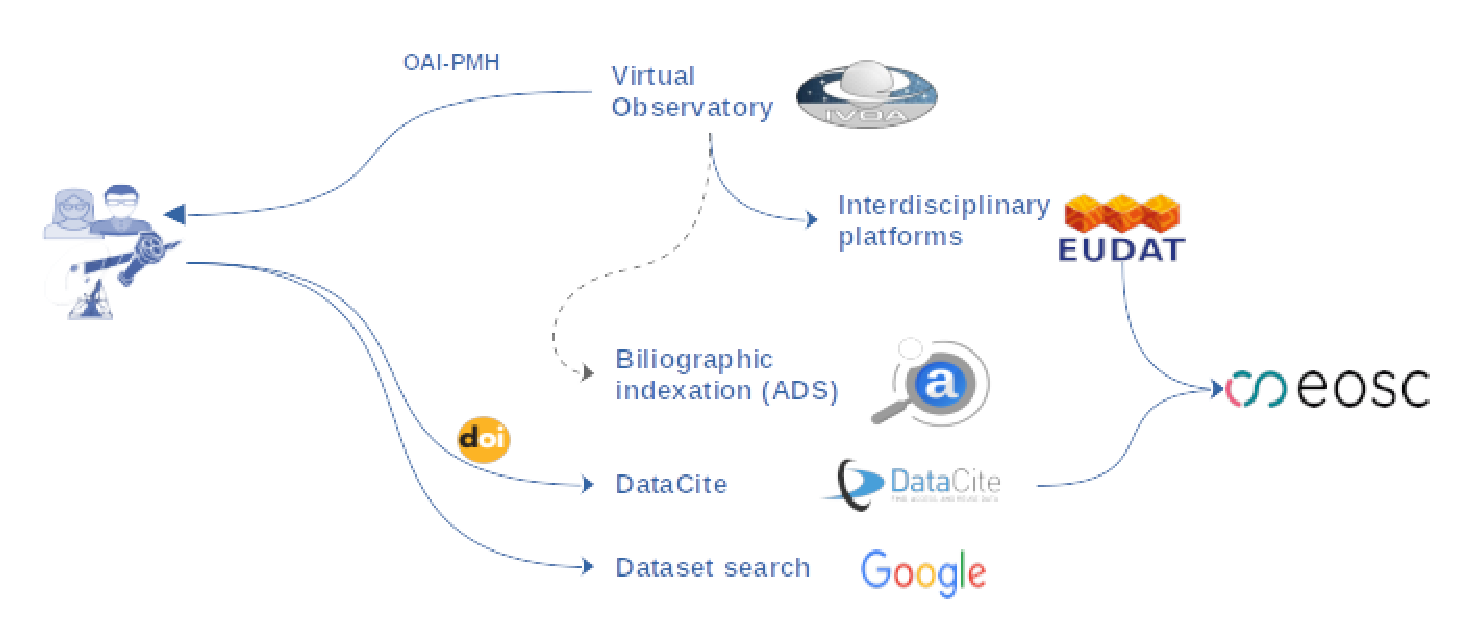
\includegraphics[width=\textwidth]{diag_dissemination2.eps}
\caption{Dissemination workflow}
\label{fig:diag-dissemination}
\end{figure}

\begin{figure}[!h]
	\centering
	\includegraphics[width=\textwidth]{schema-doi.png}
	\caption{DOI schema}
	\label{fig:doi-schema}
\end{figure}


\section{Changes from Previous Versions}

No previous versions yet.
% these would be subsections "Changes from v. WD-..."
% Use itemize environments.

\clearpage
\begin{admonition}{Note}
	All dataset citations in this document were created using BibTeX. The BibTeX for the data/service/collection DOIs is based upon the \texttt{verbatim} metadata supplied by the archive to their choice of DOI registration services as expressed by the doi2bib service\footnote{\url{https://doi2bib.org}}. The doi2bib service was selected because it does the best job protecting unfielded "author" names from complete BibTeX annihilation.
	Every other reference BibTeX came from NASA ADS\footnote{\url{https://ui.adsabs.harvard.edu/}}.
\end{admonition}

%\bibliography{ivoatex/ivoabib,ivoatex/docrepo,local}
\bibliography{DOI4Archives-gilles}
	
\end{document}
